\documentclass{beamer}
%\setbeamersize{text margin left = 0cm}
\usepackage{amsmath}
\usepackage{listings}
\usepackage{graphicx}
\usepackage{color}

 \lstset{
	%frame=tblr,
	columns=fullflexible,
	framesep=5pt,
	basicstyle=\small,
	showstringspaces=false,
	keywordstyle=\itshape\color{blue},
	%identifierstyle=\ttfamily,
	stringstyle=\color{Maroon},
	commentstyle=\color{black},
%	rulecolor=\color{Gray},
	xleftmargin=0pt,
	xrightmargin=0pt,
	breaklines = true,
	aboveskip=\bigskipamount,
	belowskip=\bigskipamount,
	%backgroundcolor=\color{LightGray!.50}
}

\title{GPU Implementation of Pb Edge Detection}
%\author{Cristian Cucu \\ \texttt{cristian\_cucu@yahoo.com}}

%\usetheme{lucid}
\begin{document}
		
	
	\frame {
		\titlepage
	}
	\frame {
		\frametitle{Outline}
		\tableofcontents
	}
	\frame {
		\frametitle{Edge Detection - Introduction}
		Edge detection is a process in which the regions where sharp color transitions in images occur are found.
		Today we would like to show how a computation intensive, memory intensive edge detection algorithm can be implemented with CUDA.
	}
	\frame{
		\frametitle{Edge Detection - Important Categories of Methods \cite{xie} }
		\begin{itemize}
			\item Pioneering Methods
			\item Information Theory and Hand Crafted Features
			\item Learning Based Methods
			\item Deep Learning Based Methods
		\end{itemize}
	}
	\frame{
	    \frametitle{Pioneering Methods}
	    \framesubtitle{Sobel Detector}
	    	Edges in the vertical and horizontal direction can be computed my convoluting the image with a vertical or horizontal Sobel mask. The operators are as follows:
	    	
	    	\begin{itemize}
	    	\item Horizontal operator: \[
	    	M_x=
	    	\begin{bmatrix}
	    	1 & 0 & -1 \\
	    	2 & 0 & -2 \\
	    	1 & 0 & -1
	    	\end{bmatrix}
	    	\]
	    	\item Vertical operator:\[
	    	M_x=
	    	\begin{bmatrix}
	    	1 & 2 & 1 \\
	    	0 & 0 & 0 \\
	    	-1 & -2 & -1
	    	\end{bmatrix}
	    	\]
	    	\end{itemize}
    	}
    \frame{
    	\frametitle{Pioneering Methods}
    	\framesubtitle{Zero Crossing Method}
	    	Zero Crossing: The image is convoluted with a second-order derivative filter, for example the Laplacian of Gaussian. In the resulted image the zero values are marked as edges.
	    	
	    	\[
	    	LoG=
	    	\begin{bmatrix}
	    	0 & 1 & 1 & 2 & 2 & 2 & 1 & 1 & 0 \\
	    	1 & 2 & 4 & 5 & 5 & 5 & 4 & 2 & 1 \\
	    	1 & 4 & 5 & 3 & 0 & 3 & 5 & 4 & 1 \\
	    	2 & 5 & 3 & -12 & -24 & -12 & 3 & 5 & 2 \\
			2 & 5 & 0 &-24 & -40 & -24 & 0 & 5 & 2 \\
			2 & 5 & 3 & -12 & -24 & -12 & 3 & 5 & 2 \\
	    	1 & 4 & 5 & 3 & 0 & 3 & 5 & 4 & 1 \\
			1 & 2 & 4 & 5 & 5 & 5 & 4 & 2 & 1 \\
			0 & 1 & 1 & 2 & 2 & 2 & 1 & 1 & 0 \\	    	
	    	\end{bmatrix}
	    	\]
	    }
 	\frame{
		\frametitle {Information Theory and Hand Crafted Features \cite{konishi}}
		\framesubtitle {Statistical Edges}
		The methods calculates the multi-dimensional probability densities $P(\phi(I(x) | edge))$ and $P(\phi(I(x) | not-edge))$, where $\phi$ is a filter applied in the image I at the position x. A pixel in the image is on an edge when $\frac{P(\phi(I(x) | edge))}{P(\phi(I(x) | not-edge))} > T$ , where T is a suitably chosen threshold. The probability density functions are modelled as histograms.
	}
    \frame{
		\frametitle {Information Theory and Hand Crafted Features}
		\framesubtitle {Pb - Probability of Boundary - Edge Detector}
		For each point of an image and each orientation an edge value is computed as follows:
		\begin{itemize}
			\item A disc of radius R centered at the point is superimposed on the image
			\item The disc is divided into two half discs by a diameter with the chosen orientation
			\item For the image points in each half disc the histogram of intensities in the image (other features like texture, different color channel values are possible) are computed
			\item The gradient at the chosen point, with the given edge orientation, and disc radius is computed as the $\chi$-square distance between the two histograms computed
		\end{itemize}
	}
	\frame{
		\frametitle {Information Theory and Hand Crafted Features}
		\framesubtitle {Multiscale Pb - Part 1}
		A multiscale Pb detector for each orientation can be obtained with the following formula
		
		\[ mPb(x,y,\theta) = \sum_{s}^{} \sum_{i}^{}\alpha_{i,s} G_{i,\sigma(i,s)}(x,y,\theta) \]
		\begin{itemize}
			\item i represents the channel used (L, a, b or texture channel)
			\item s represents scales
			\item $G_{i,\sigma(i,s)}(x,y,\theta)$ represents the probability of boundary gradient in the image channel i, at the disc radius $\sigma(i,s)$, at the point (x,y) in image and with the orientation $\theta$
		\end{itemize}
	}

	\frame{
	\frametitle {Information Theory and Hand Crafted Features}
	\framesubtitle {Multiscale Pb - Part 2}
	In order to obtain orientation independent multiscale Pb edges the following is computed:
		\[ mPb(x,y) = \max\limits_{\theta} mPb(x,y,\theta)\]
	The edges are then thinned with a non-maximum suppression term.
	The parameters $\alpha_{i,s}$ are computed with a gradient ascent method on the training images.
		
	}	

	\frame{
	\frametitle {Information Theory and Hand Crafted Features}
	\framesubtitle {Global Pb - Part 1}
	To account for bigger context in the image a global component is added local component (mPb) in the gPb algorithm. This component is constructed as follows: 
	\begin{itemize}
		\item A square matrix W with dimension equal to the number of pixels in the image is defined as follows:
		\begin{itemize}
		 \item an influence radius r is chosen
		 \item when the distance between pixels i and j is smaller or equal r, : \[ W_{ij} = exp(-\max\limits_{p \in \bar{ij}} \frac{mPb(p)}{\rho})\], $\bar{ij}$ is the segment connecting i and j, 
		 \item when the distance between pixels i and j is equal than \[W_{ij} = 0\]
		 \end{itemize}
		\item A square matrix D as follows: \[ D_{ii} = \sum_{j} W_{ij}\]
		
	\end{itemize}	
	} 

	\frame{
	\frametitle {Information Theory and Hand Crafted Features}
	\framesubtitle {Global Pb - Part 2}
	\begin{itemize}
		\item A generalized eigenvalue problem is solved \[ (D - W) v = \lambda D v\]
		\item The eigenvectors $v_{n}$ associated with the n smallest non-trivial eigenvalues are taken. Each of them contains a value for each of image pixels. From each vector an image is recreated and gradient images with the gradient operator with orientation $\theta$ is computed. 
		\item The resulting global edges follow the formula: \[ sPb(x,y,\theta) = \sum_{k=1}^{n}\frac{1}{\sqrt{\lambda_{k}}} \nabla_{\theta} v_{k}(x,y) \]  
		
		
	\end{itemize}	
	} 

	\frame {
	\frametitle{CUDA - Introduction}
	\begin{itemize}
		\item CUDA is a framework developed by NVIDIA for programming with the GPU. 
		\item Supported graphic cards are the NVIDIA GPUs. 
		\item The programming language is an extension of C.
	\end{itemize}
	}

	\frame {
	\frametitle{CUDA - Programming model}
	\begin{itemize}
		\item Two main entities: host (CPU) and device (GPU).The host organizes data transfer to the GPU and starts the parallel operations on them.
		\item GPU can have thousands of processing units on which multiple threads are running.
		\item Data transfer from CPU to GPU is slow and must be minimized as much as possible.
	\end{itemize}
	}
	\frame {
	\frametitle{CUDA - Simple Program Structure}
	The structure of a CUDA program is as follows:
	\begin{itemize}
		\item Copy data from CPU to GPU memory
		\item Invoke kernels to operate on the data stored in the GPU memory
		\item Copy data back from GPU to CPU
	\end{itemize}
}

	\begin{frame} [fragile] 
	\frametitle{Sum of two vectors with CUDA - Part 1}
	Initialize pointers to device memory, copy input data from host to device:
	\begin{lstlisting}
	void addWithCuda(int* c, const int* a, const int* b, int size) {
	int* dev_a = nullptr;
	int* dev_b = nullptr;
	int* dev_c = nullptr;
	
	cudaMalloc((void**)&dev_c, size * sizeof(int));
	cudaMalloc((void**)&dev_a, size * sizeof(int));
	cudaMalloc((void**)&dev_b, size * sizeof(int));
	
	cudaMemcpy(dev_a, a, size * sizeof(int), cudaMemcpyHostToDevice);
	cudaMemcpy(dev_b, b, size * sizeof(int), cudaMemcpyHostToDevice);
	\end{lstlisting}
	\end{frame}
	
	
	\begin{frame} [fragile] 
	\frametitle{Sum of two vectors with CUDA - Part 2}
	Execute the parallel code, synchronize the threads, copy the results back to host,
	free memory on the device:
	\begin{lstlisting}
	addKernel<<<2, (size + 1) / 2>>>(dev_c, dev_a, dev_b, size);
	
	cudaDeviceSynchronize();
	
	cudaMemcpy(c, dev_c, size * sizeof(int), cudaMemcpyDeviceToHost);
	
	cudaFree(dev_c);
	cudaFree(dev_a);
	cudaFree(dev_b);
	}
	\end{lstlisting}
	\end{frame}
	
	\begin{frame} [fragile] 
	\frametitle{Sum of two vectors with CUDA - Part 3}
	Parallel kernel executed cooperatively by multiple threads:
	\begin{lstlisting}
	__global__ void addKernel(int* c, const int* a, const int* b, int size) {
	int i = blockIdx.x * blockDim.x + threadIdx.x;
	if (i < size) {
	c[i] = a[i] + b[i];
	}
	}
	
	\end{lstlisting}
	\end{frame}

	\begin{frame}
	\hspace*{1cm}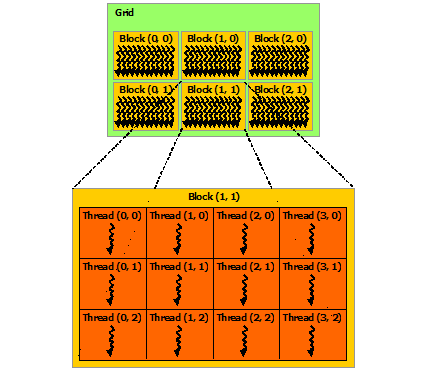
\includegraphics[scale=0.8]{grid-of-thread-blocks.png}
	\end{frame}

	\frame {
	\frametitle{Allocate Host and Device Memory }
	\begin{itemize}
		\item GPU memory is managed with function calls similar to C functions: cudaMalloc, cudaMemcpy, cudaMemset, cudaFree.
		\item It is illegal to access device memory in host code and host memory in device code. There exists a mode of memory access called the Unified Memory Model where code can access both device and host memory at the same time. (TODO??)
	\end{itemize}
}

	\begin{frame}  
	\frametitle{Implement a Kernel}
	\begin{itemize}
		\item When a kernel has been launched, control is returned immediately to the host, which can perform asynchronously other tasks.
		\item After the kernel has been started one can call cudaDeviceSynchronize in order to wait for all threads to finish and synchronize with the host thread.
		\item Kernel launch parameters are as follows: 	$<<< Dg, Db, Ns, S >>>$
			%where:
			\begin{itemize}
				\item Dg - the dimension of the grid of blocks
				\item Db - the dimension of the block
				\item Ns - shared memory allocated for each block
				\item S - the associated stream (optional)
			\end{itemize}
	\end{itemize}
	\end {frame}

	\frame {
	\frametitle{Thread Organition in CUDA}
	\begin{itemize}
		\item Threads launched by the same kernel are organized in a 3D structure called grid. All threads in a grid share the same global memory space.
		\item Each grid element can contained another 3D structure of threads called a block. Threads in the same block can cooperate with each other by using
		\begin{itemize}
			\item Block-local synchronization
			\item Block-local shared memory
		\end{itemize}
		\item To distinguish them from each other threads use two identifiers:
		\begin{itemize}
			\item blockIdx (block index within a grid)
			\item threadIdx (thread index within a block)
		\end{itemize}
	\end{itemize}
}

	\frame {
	\frametitle{Host Memory and Device Memory}
	\begin{itemize}
		\item Two main entities: host (CPU) and device (GPU).The host organizes data transfer to the GPU and starts the parallel operations on them.
		\item GPU can have thousands of processing units on which multiple threads are running.
		\item Data transfer from CPU to GPU is slow and must be minimized as much as possible.
		Today we would like to show how a computation intensive, memory intensive edge detection algorithm can be implemented with CUDA.
	\end{itemize}
}


	\frame {
	\frametitle{For Loop with CUDA - 2D}
	\begin{itemize}
		\item Two main entities: host (CPU) and device (GPU).The host organizes data transfer to the GPU and starts the parallel operations on them.
		\item GPU can have thousands of processing units on which multiple threads are running.
		\item Data transfer from CPU to GPU is slow and must be minimized as much as possible.
		Today we would like to show how a computation intensive, memory intensive edge detection algorithm can be implemented with CUDA.
	\end{itemize}
}

	\begin{frame} [fragile] 
	\frametitle{Pb - single thread version - 1}
	\begin{lstlisting} [language=C++]
	HistoVect histograms;
	initializeHistoRange(histograms, 0, m_Scale + 1);	

	for (int i = 0; i < m_SingleChannelImage.rows + 2 * m_Scale; ++i) {
		for (int j = 0; j < m_SingleChannelImage.cols + 2 * m_Scale; ++j) {
		int val = bufImg.at<unsigned char>(i, j);	
		addToHistoMaps(histograms, val, i, j);
		}
		calculateGradients(histograms, i);
		deleteFromHistoMaps(histograms, i);
	}
	\end{lstlisting} 
	\end{frame}

	\frame {
	\frametitle{Pb - single threaded version - 2}
	How are the histograms stored ? 
}

	\frame {
	\frametitle{Pb - CUDA version}
	Edge detection is a process in which the regions where sharp color transitions in images occur are found.
	Today we would like to show how a computation intensive, memory intensive edge detection algorithm can be implemented with CUDA.
}

	\begin{thebibliography}{9}		
		\bibitem{liu} 
		Yun Liu, Ming-Ming Cheng, Deng-Ping Fan, Le Zhang, Jia-Wang Bian, and Dacheng Tao, Fellow, IEEE
		\textit{Semantic Edge Detection with Diverse Deep Supervision} 
		IEEE Transactions on Pattern Analysis and Machine Intelligence, 2018
		\bibitem{xie}
		Saining Xie, Zhuowen Tu, Holistically-Nested Edge Detection, arXiv 2015
		\bibitem{konishi}
		Scott Konishi, Alan L. Yuille, James M. Coughlan, and Song Chun Zhu
		\textit{Statistical Edge Detection: Learning and Evaluating Edge Cues}
		IEEE Transactions on Pattern Analysis and Machine Intelligence, Vol. 25, No. 1, January 2003

	\end{thebibliography}

\end{document}




